%
% tests
% @author Tobias Weber <tweber@ill.fr>
% @date aug-2021
% @license see 'LICENSE' file
%

\chapter{Test Tools and Unit Tests}
\label{ch:tests}
Due to a rapid increase in its complexity over time, the software of this work 
necessitated a multi-tiered testing strategy during development, including test programs and unit tests.
Even after having finished the critical phases of development, the programs which are 
presented in this chapter serve to ensure that the software and its parts continue to work as intended. 
Problems that may arise can be rapidly analysed using the simplified environments these tools provide.

Before having being integrated into the main library or the GUI program, each essential function was tested 
separately. This was done either via small test programs or via dedicated unit tests, which are discussed in 
section \ref{sec:unit_tests}.
Integration tests of algorithms, where collections of functions are tested how and if they work together, 
were performed using larger bespoke test tools, which implemented a simplified versions of the functionality 
of the main programs. These are described in section \ref{sec:tests_tools}.



\section{Test tools}
\label{sec:tests_tools}
First, we describe the collection of tools that served in testing aspects of the main path-finding algorithm.
These tools share a common \textit{Qt}-based \cite{web_Qt} GUI codebase and are similar in their usage.
They all use the \lstinline[language=C++]|QGraphicsScene| class \cite{web_QGraphicsScene} and through that
allow a dynamic manipulation of their respective geometrical objects using the mouse. 
Calculations and results are automatically updated once the user changes the geometrical scenes.

Early versions of these tools were originally created in 2020 as preparation for the exam in the Algorithmic
Geometry course, the original repository can be found on-line at \url{https://github.com/t-weber/geo}. 
Afterwards, these programs were further developed for their current purpose during the present work.


\subsection{Line segments tool}
\label{sec:tests_linesegs}
The line segment tool (Fig. \ref{fig:linesgui}), whose code can be found in the file 
\lstinline|./src/tools/lines.cpp| of the source repository, 
performs several kinds of computations to test the line-based algorithms that are used in the core module.

The most important of these is the calculation of line segment Voronoi diagram bisectors as shown in 
Fig. \ref{fig:linesgui} (a), please also refer to chapter \ref{sec:voro_ls}.
To that end, it uses two different backend libraries between which the user can switch dynamically in
the program. These libraries are \textit{Boost.Polygon}'s Voronoi module \cite{web_boost_polygon_voronoi} for one
and \textit{OpenVoronoi} \cite{web_openvoronoi} for the other.
The correctness of the calculation is furthermore checked by iterating the points of the $\mathbb{R}^2$ plane
on a grid and testing to which line segment they are closest. These are the coloured regions in Fig. \ref{fig:linesgui} (a).
The line segment tool can load the regions of the angular configuration space that are calculated in the main
program (chapter \ref{sec:line_seg_generation}), and was used for debugging purposes in its development and
for testing different approaches to the algorithms used in the main program.

Another calculation the line segment tool performs and which is shown in Fig. \ref{fig:linesgui} (b), is the 
calculation of trapezoidal maps (chapter \ref{sec:pointrobot_sector}), which are calculated according to the 
algorithm given in Ref. \cite[Ch. 6, pp. 121-146]{Berg2008}.
The purpose of this was for early testing which sector-based method would be most suitable
for path-mesh building. The trapezoid maps were deemed infeasible and were ruled out after
these tests.

The third calculation that was tested in this tool is the sweep-based intersection of line segments which
is used in the main algorithm for intersections checks between polygons, as has been discussed in 
chapter \ref{sec:angular_config_space}.
The implementation is based on the algorithm given in Ref. \cite[pp. 69-80]{FUH_geo2020}.

\begin{figure}[h]
	\centering
	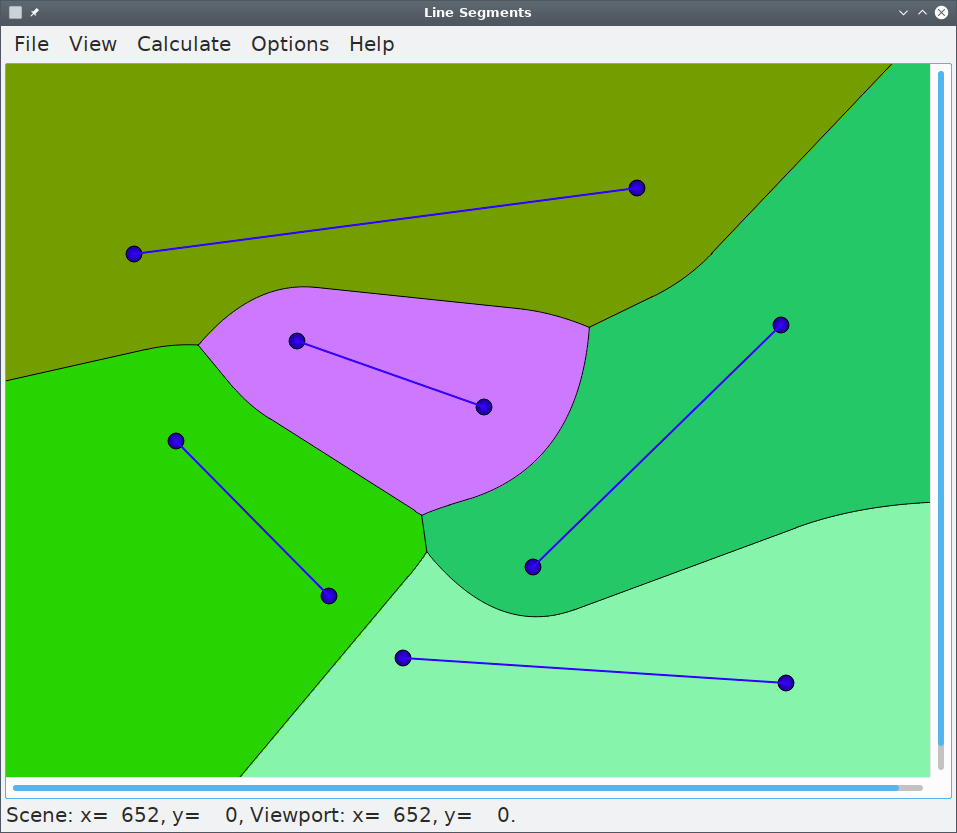
\includegraphics[width = 0.49 \textwidth]{figures/linesgui_voro}
	\hspace{0.05cm}
	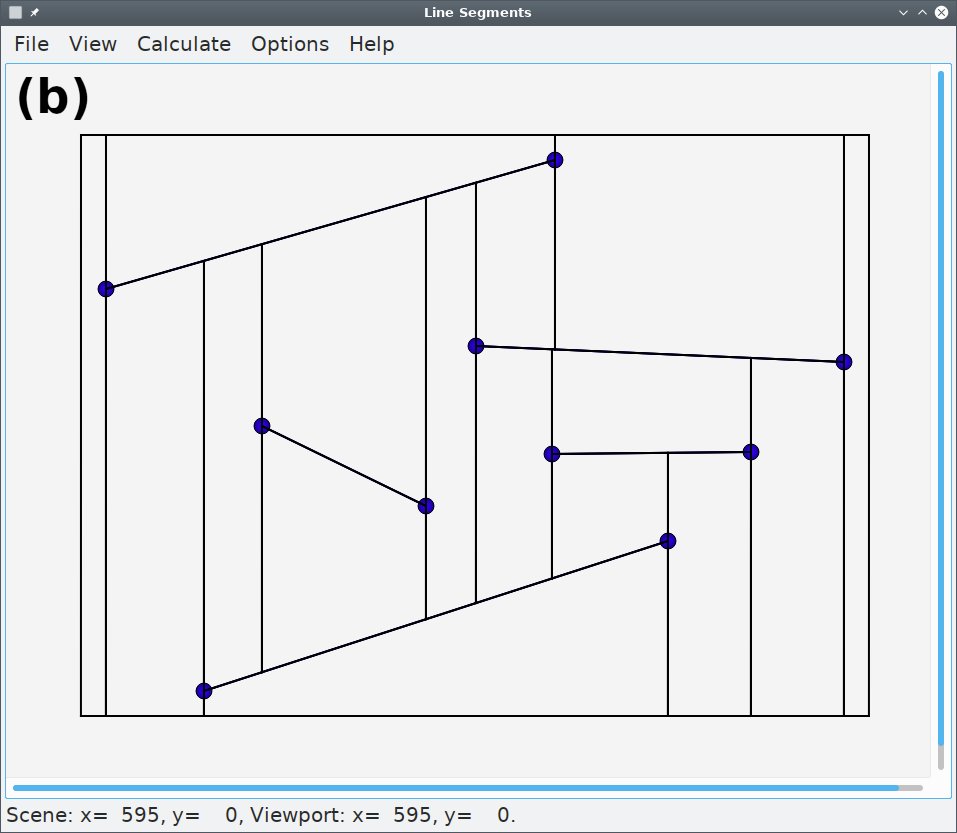
\includegraphics[width = 0.49 \textwidth]{figures/linesgui_trapezoid}

	\vspace{0.25cm}
	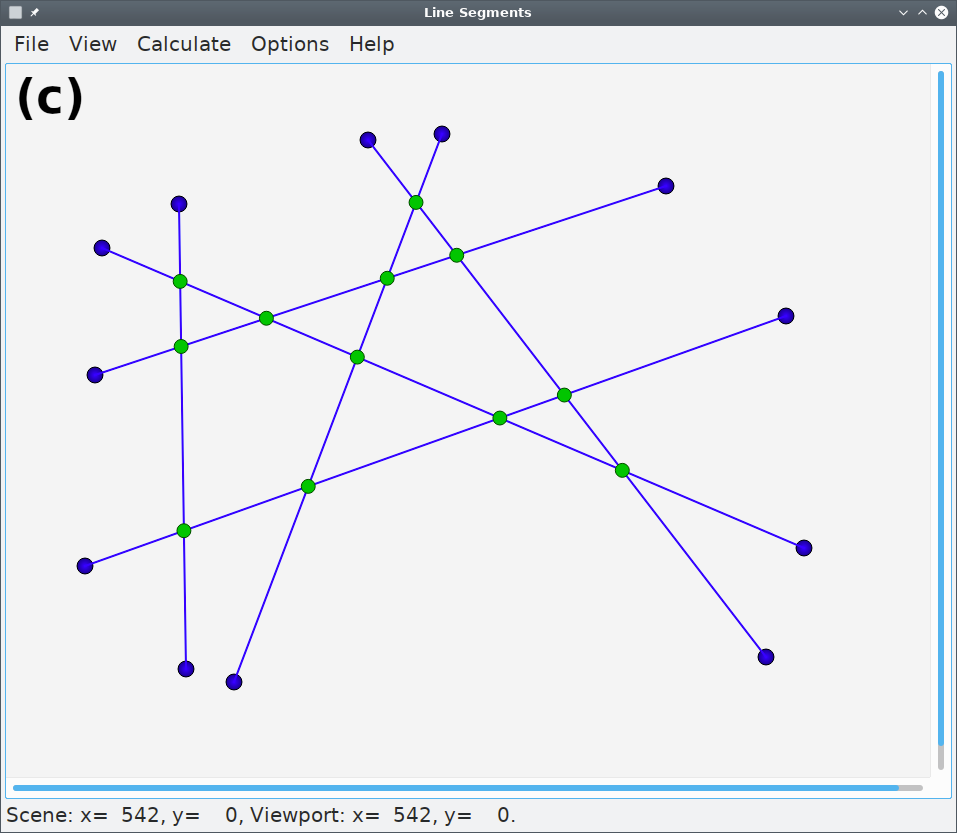
\includegraphics[width = 0.49 \textwidth]{figures/linesgui_inters}
	\caption[Line segments tool.]{Line segments tool.
		This program allows the dynamic calculation of
		(a) line segment Voronoi regions (coloured) and bisectors (black lines),
		(b) trapezoidal maps, and
		(c) sweep-based points of intersection (green points).
		Line segment vertices can be inserted, deleted and moved using the mouse.
		\label{fig:linesgui}}
\end{figure}



\subsection{Polygon tool}
The next tool performs calculations and tests on polygonal algorithms. 
Its source code can be found in the file \lstinline|./src/tools/poly.cpp|.

The main purpose of the polygon tool is the testing of the algorithm used for splitting concave 
polygonal regions into convex sub-regions that is used in building the path mesh in chapter \ref{sec:convex_regions}. 
Fig. \ref{fig:polygui} (a) shows a screenshot of a test run of the algorithm on a much simpler
polygonal region than what is calculated in the main program. The polygonal splitting algorithm 
itself is based on the description from Ref. \cite{Hegazy2014}.
Another function of the tool is the calculation of the visibility kernel \cite{TODO} of a 
polygonal region, see Fig. \ref{fig:polygui} (b).


\begin{figure}[h]
	\centering
	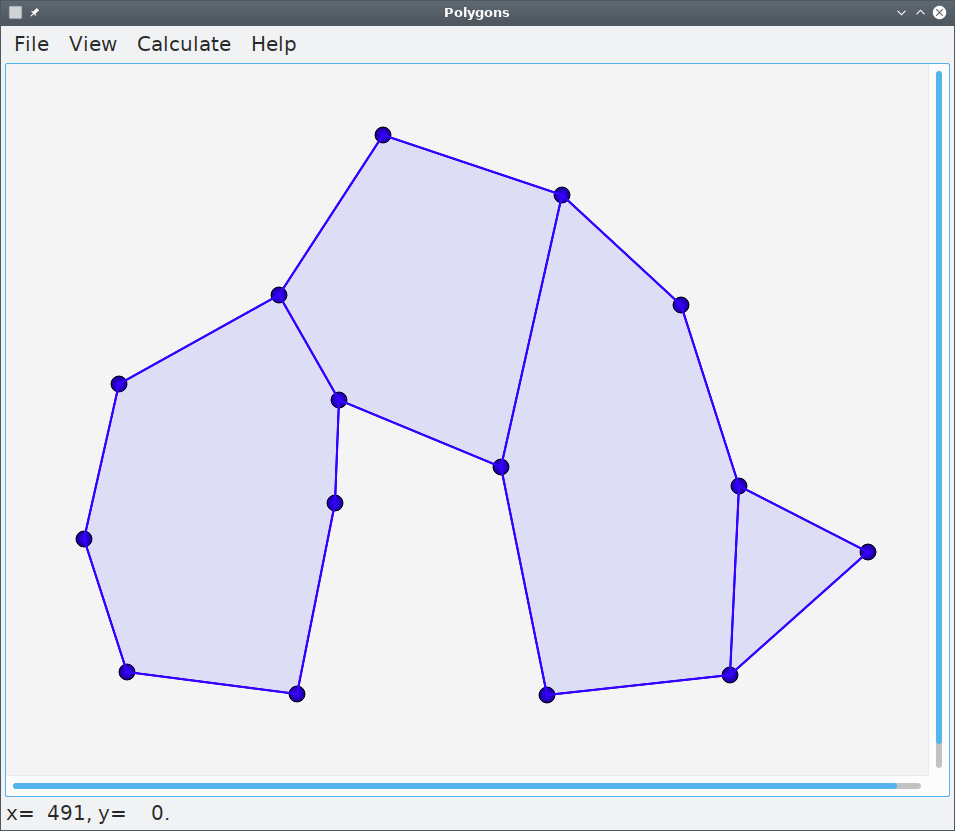
\includegraphics[width = 0.49 \textwidth]{figures/polygui_convex}
	\hspace{0.05cm}
	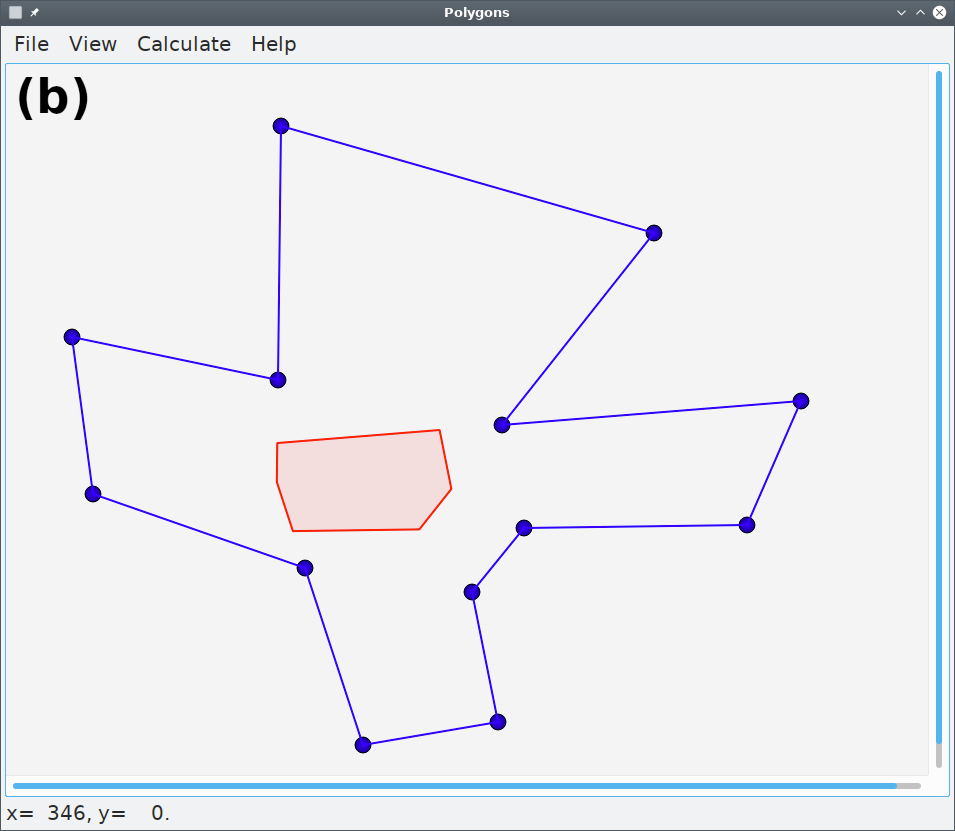
\includegraphics[width = 0.49 \textwidth]{figures/polygui_kernel}
	\caption[Polygon tool.]{Polygon tool.
		This program calculates the
		(a) convex sub-regions of a concave polygon, and
		(b) the visibility kernel (red) of a polygonal region.
		Polygon vertices can be inserted, deleted and moved using the mouse, updates
		are performed dynamically.
		\label{fig:polygui}}
\end{figure}



\subsection{Convex hull tool}
\label{sec:tests_hull}
The final tool performs calculations on collections of vertices.

Its main functionality consists of determining the convex hull \cite[Ch. 11, pp. 243-258]{Berg2008}, 
the Voronoi diagrams \cite[Ch. 7, pp. 147-171]{Berg2008}, 
as well as the Delaunay triangulation \cite[Ch. 9, pp. 191-218]{Berg2008} 
of the given set of vertices. This is shown in Fig. \ref{fig:hullgui} (a).
A secondary feature, depicted in Fig. \ref{fig:hullgui} (b), is the calculation of 
the minimal spanning tree between the vertices using Kruskal's algorithm \cite[pp. 265-268]{Erickson2019}.

For calculating the convex hull, several different algorithms have been implemented,
which can be selected in the program's ``backend'' menu.
These backends comprise the contour polygon method \cite[Ch. 3.1.5, pp. 125-128]{FUH_geo2020},
the iterative incremental calculation \cite[Ch. 3.1.3, pp. 117-123]{FUH_geo2020}, as well as the 
recursive divide-and-conquer method \cite[Ch. 3.1.4, pp. 123-125]{FUH_geo2020}, 
which have been implemented according to the pseudo-codes and descriptions given
in the respective references.
One further backend includes calculation via the \textit{QHull} library \cite{web_qhull}.
Not surprisingly, all backends yield the same results.

Similarly to the convex hull calculation, the calculation of the Delaunay triangulation
also supports multiple backend algorithms.
Among them are the incremental method \cite[Ch. 6.2, pp. 269-282]{FUH_geo2020}, 
delegating calculations \textit{QHull} \cite{web_qhull}, 
and third, the parabolic transformation \cite[Ch. 6.5, pp. 298-300]{FUH_geo2020}, 
which also partially uses \textit{QHull}, namely to calculate the three-dimensional 
convex hull of the transformed problem.

\begin{figure}[h]
	\centering
	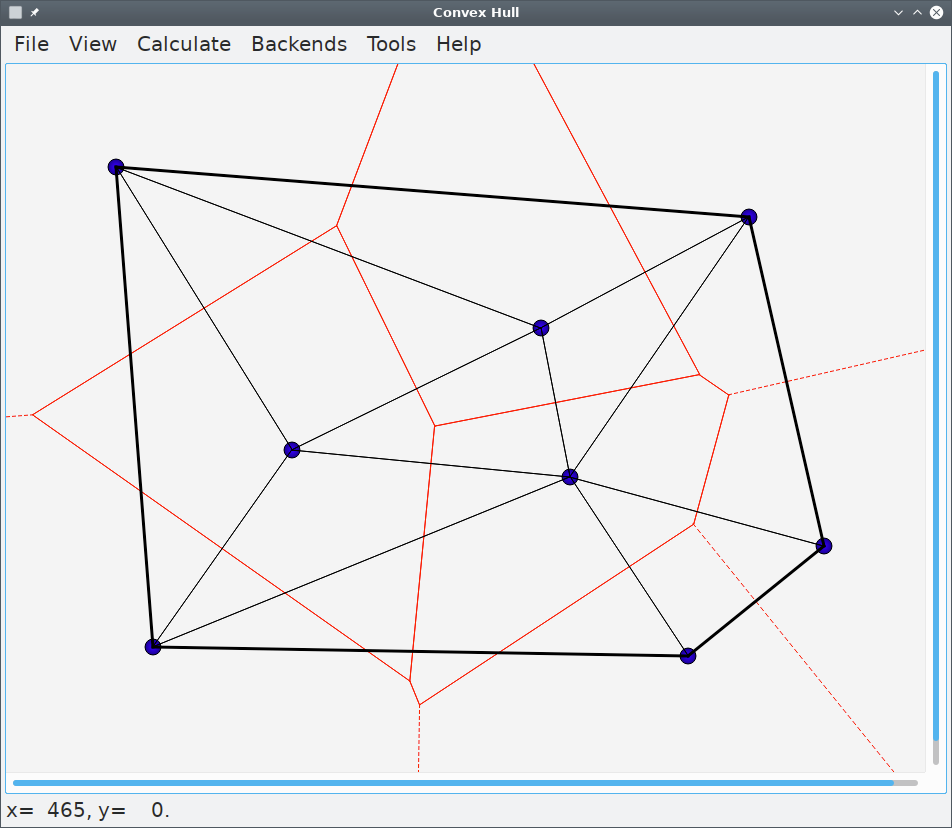
\includegraphics[width = 0.49 \textwidth]{figures/hullgui_voro}
	\hspace{0.05cm}
	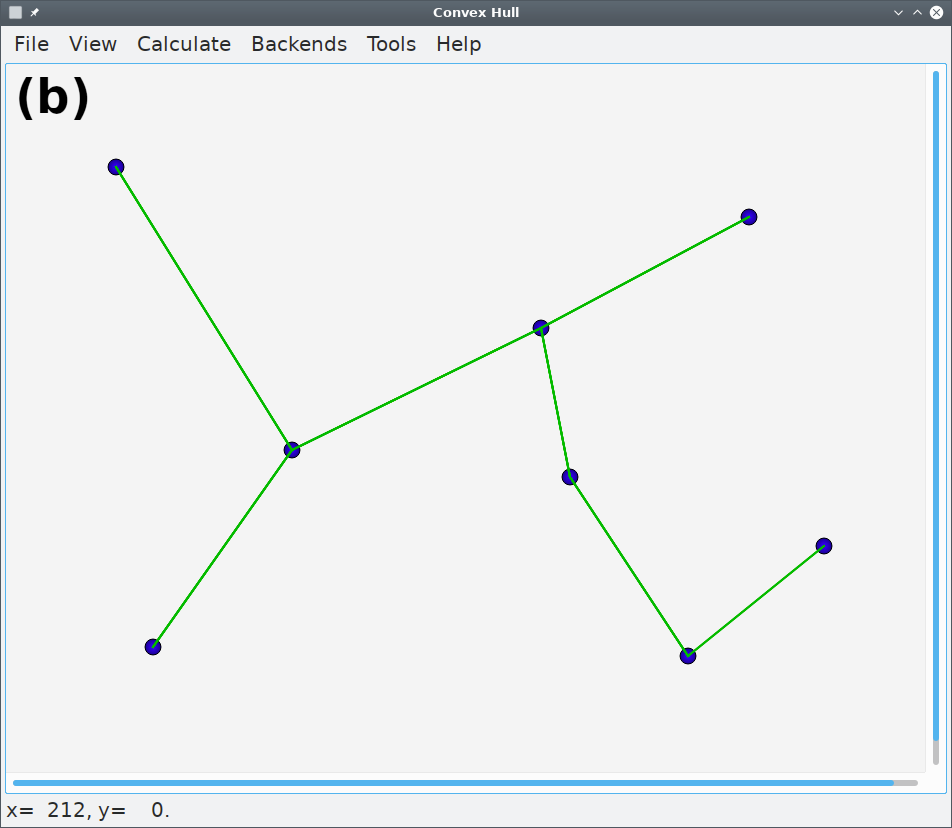
\includegraphics[width = 0.49 \textwidth]{figures/hullgui_kruskal}
	\caption[Convex hull tool.]{Convex hull tool.
		This program calculates 
		(a) the convex hull (thick black lines), the Voronoi diagram (red lines), 
			the Delaunay triangulation (thin black lines), as well as
		(b) Kruskal's minimum spanning tree (green lines)
		of a collection of vertices.
		As with the other test tools, the vertices can be inserted, deleted and moved 
		using the mouse, updates are performed dynamically.
		\label{fig:hullgui}}
\end{figure}




\section{Unit tests}
\label{sec:unit_tests}
A unit test tests if a given set of inputs to a function gives an expected set of outputs.
Testing an algorithm containing several function calls also allows to check if a set of invariants
is fulfilled during the algorithm run, meaning between function calls.
Possible checks can either be fixed input values which are tested against known output values,
or random inputs for which the correct output is calculated independently using a different 
method than the one being tested, or even an external program.
A comprehensive description of unit testing is given in Ref. \cite[Ch. 3, pp. 73-105]{FUH_prog2019}.

Unit tests allow to spot an error for which they are specifically designed. Conversely, they cannot 
prove that a software is free of errors. Such a feat would be the task of software
verification \cite[Ch. 5, pp. 117-144]{Berghammer2017}, which is complicated, if not impossible for
software systems of a certain size and complexity.
Software verification uses proofs via Hoare logic, which splits the program into its primitive
operations (e.g. assignments, conditions, loops) \cite[pp. 118-119]{Berghammer2017}, formulates
a set of axioms and derivation rules consisting of pre- and post-conditions for these primitive operations
\cite[pp. 122]{Berghammer2017}, reduces the complex program into these axioms \cite[pp. 123]{Berghammer2017},
and finally either proofs the partial or the total correctness of the program.
The former says that if the pre-condition is valid, the post-condition is also valid after running the
program, the latter means that the post-condition follows from the pre-condition and the execution
of the program \cite[pp. 121]{Berghammer2017}.

For the present software, unit tests of isolated functions and algorithms were performed using the 
C++ library \textit{Boost.Test} \cite{web_boost_test}.
In \textit{Boost.Test}, test modules are defined per unit test file, which contains one or more test cases.
These test cases can also be configured to create different instances of template functions using
different template arguments. The body of a test case contains a block of normal C++ code.
In the C++ code, conditions and invariants are tested using the 
\lstinline[language=C++]|BOOST_TEST()| macro. Each successful or non-successful evaluation
of the macro is registered by \textit{Boost.Test} and reported in a final summary.
